\chapter{विद्युत-रासायनिक सेल और विद्युत-अपघटन}\label{ch:g12:cells-and-electrolysis}

सर्दियों की एक शाम फ़ोन 1 \% दिखाता है और बंद हो जाता है। रात भर चार्ज पर लगा रहने के बाद
सुबह तक वह फिर भर जाता है। उसकी बैटरी के भीतर वही \omterm{def:g7:chemical-reactions:reaction}{रासायनिक अभिक्रिया}
दिन में एक दिशा में चलती है, विद्युत ऊर्जा देती हुई, और रात में चार्जर उसे
दूसरी दिशा में धकेलता है। कोई \omterm{def:g11:redox:reaction}{अपचयोपचय अभिक्रिया} तब विद्युत का स्रोत बन जाती है
जब उसके \omterm{def:g9:inside-the-atom:nucleus}{इलेक्ट्रॉनों} को एक तार से होकर गुज़रने पर मजबूर किया जाए;
और किसी विलयन से धकेली गई विद्युत ऐसी \omterm{def:g11:redox:reaction}{अपचयोपचय अभिक्रिया} करा सकती है
जो अपने आप कभी नहीं होती।

\begin{recall}
\omterm{def:g11:redox:oxidant}{ऑक्सीकारक} \omterm{def:g9:inside-the-atom:nucleus}{इलेक्ट्रॉन} ग्रहण करते हैं, \omterm{def:g11:redox:oxidant}{अपचायक} उन्हें खोते हैं; \omterm{def:g11:redox:couple}{अर्ध-समीकरण}, \omterm{def:g11:redox:couple}{अपचयोपचय
युग्म} और \omterm{def:g11:redox:reaction}{अपचयोपचय अभिक्रियाएँ} (\cref{ch:g11:redox})। कोई निकाय तब तक विकसित होता है जब तक
$Q = K$ न हो जाए (\cref{ch:g12:equilibrium})। \omterm{def:g9:ions:ion}{आयनों} के विलयन चालन करते हैं
(\cref{ch:g9:ions}); \omterm{def:g10:the-mole:amount}{मोल} और \omterm{def:g10:the-mole:avogadro}{आवोगाद्रो स्थिरांक}
(\cref{ch:g10:the-mole})।
\end{recall}

\begin{omfigure}
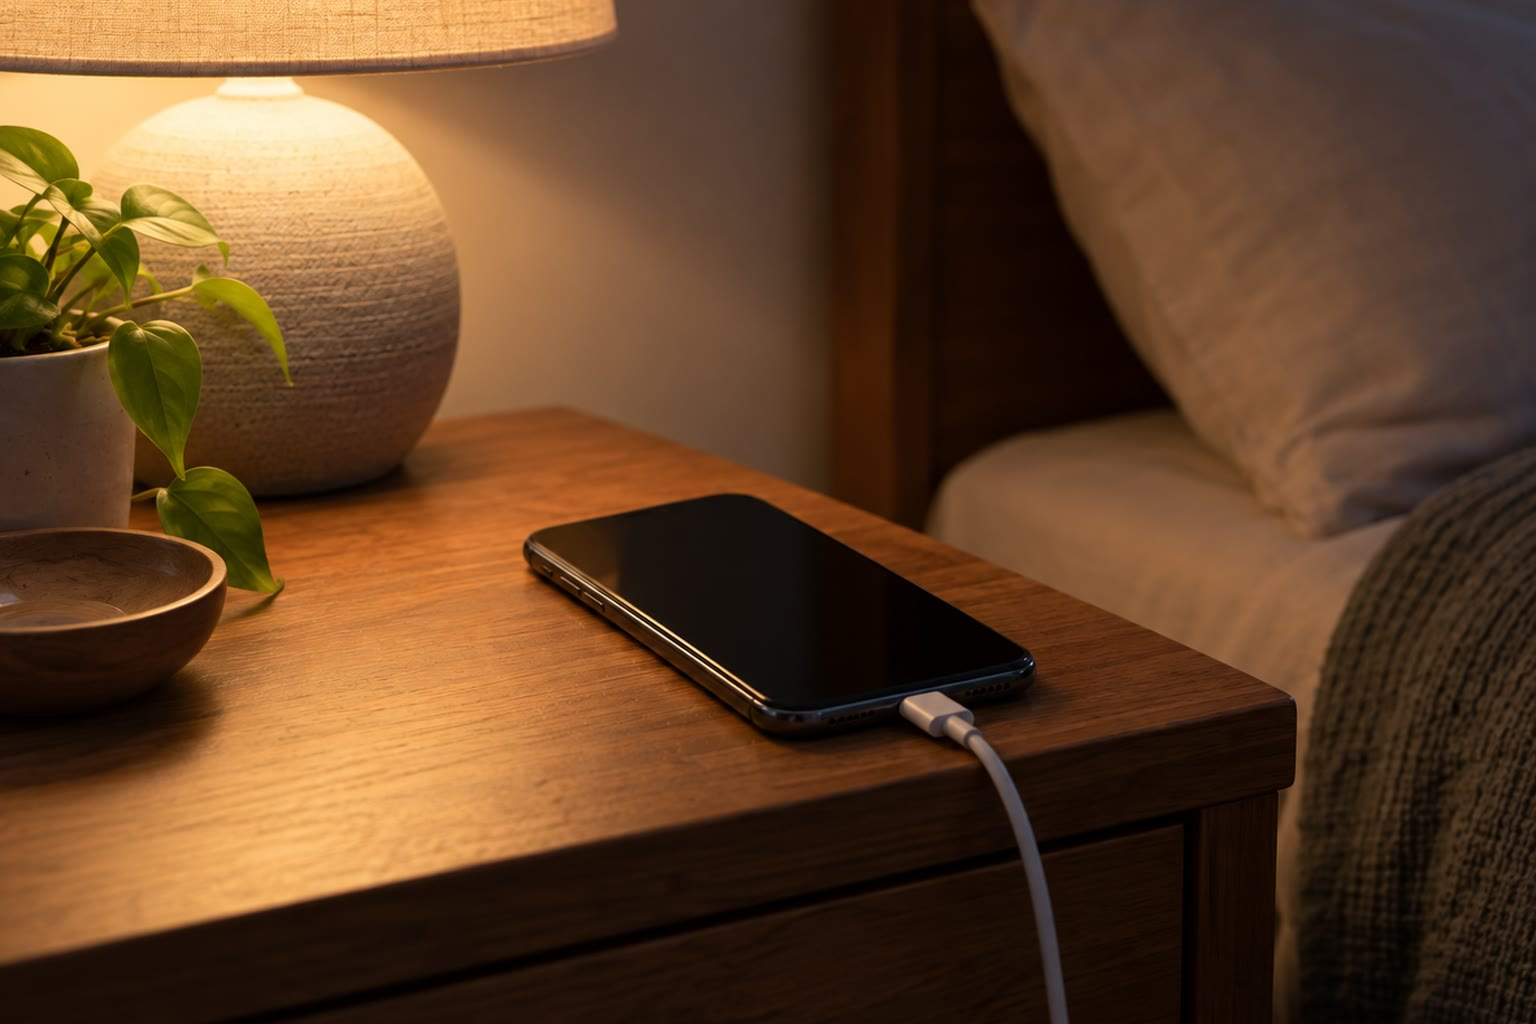
\includegraphics[width=0.45\linewidth]{images/book1/ai/g12-phone-charging.jpg}

{\small फ़ोन चार्ज करना: रात भर उलटी दिशा में धकेली गई एक अभिक्रिया।}
\end{omfigure}

\section{दो भागों में बँटी एक अपचयोपचय अभिक्रिया}

जब जस्ते की पट्टी कॉपर सल्फ़ेट विलयन में डुबोई जाती है, तो पट्टी की सतह पर जस्ता ऑक्सीकृत होता है
और कॉपर \omterm{def:g9:ions:ion}{आयन} अपचयित होते हैं,
\ce{Zn + Cu^{2+} -> Zn^{2+} + Cu}: \omterm{def:g9:inside-the-atom:nucleus}{इलेक्ट्रॉन} \omterm{def:g9:periodic-table-first-look:metal}{धातु} से सीधे
\omterm{def:g9:ions:ion}{आयनों} तक जाते हैं, और ऊर्जा थोड़ी-सी ऊष्मा के रूप में नष्ट हो जाती है। दोनों
अर्धों को अलग कीजिए, और उन्हें एक तार से जोड़िए: अब \omterm{def:g9:inside-the-atom:nucleus}{इलेक्ट्रॉनों} को
तार से होकर जाना पड़ता है, और रास्ते में वे एक बल्ब जला सकते हैं।

\begin{definition}[विद्युत-रासायनिक सेल, अर्ध-सेल, लवण सेतु]\label{def:g12:cells-and-electrolysis:cell}
\emph{विद्युत-रासायनिक सेल}\index{विद्युत-रासायनिक सेल} एक ऐसी \omterm{def:g11:redox:reaction}{अपचयोपचय अभिक्रिया} से
विद्युत ऊर्जा उत्पन्न करता है जिसका \omterm{def:g11:redox:oxidation}{ऑक्सीकरण} और \omterm{def:g11:redox:oxidation}{अपचयन}
दो अलग-अलग कक्षों में होते हैं। हर कक्ष, अपने \omterm{def:g9:ions:ion}{आयनों} के विलयन में डूबा
एक \omterm{def:g9:periodic-table-first-look:metal}{धातु} इलेक्ट्रोड, एक
\emph{अर्ध-सेल}\index{अर्ध-सेल} है। \emph{लवण सेतु}\index{लवण सेतु},
\omterm{def:g9:ions:ion}{आयनों} के विलयन में भीगी एक नली या कागज़ की पट्टी, दोनों
विलयनों को जोड़ता है और उन्हें अलग रखते हुए परिपथ पूरा करता है।
\end{definition}

\begin{definition}[ऐनोड, कैथोड]\label{def:g12:cells-and-electrolysis:anode}
जिस इलेक्ट्रोड पर \omterm{def:g11:redox:oxidation}{ऑक्सीकरण} होता है, वह
\emph{ऐनोड}\index{ऐनोड} है; जिस इलेक्ट्रोड पर \omterm{def:g11:redox:oxidation}{अपचयन} होता है,
वह \emph{कैथोड}\index{कैथोड} है।
\end{definition}

\begin{omfigure}
\begin{tikzpicture}[font=\small, scale=1.25]
  \pic[transform shape] at (0,0) {beaker={0.7}{black!6}};
  \pic[transform shape] at (4,0) {beaker={0.7}{cyan!70!blue!35}};
  \pic[transform shape] (zn) at (-0.3,0.25) {electrode={black!30}};
  \pic[transform shape] (cu) at (4.3,0.25) {electrode={orange!70!brown}};
  \pic[transform shape] at (0.35,0.6) {saltbridge={3.3}};
  \pic[transform shape] (v) at (2,3.9) {meter={1.10 V}};
  \draw[black!70, thick] (zn-top) |- (1.0,3.4) -| (v-a);
  \draw[black!70, thick] (cu-top) |- (3.0,3.4) -| (v-b);
  \draw[->, omProp, very thick] (0.2,3.55) -- (1.0,3.55);
  \draw[->, omProp, very thick] (3.0,3.55) -- (3.8,3.55);
  \node[omProp, font=\footnotesize] at (0.6,3.75) {$e^-$};
  \node[omProp, font=\footnotesize] at (3.4,3.75) {$e^-$};
  \node[anchor=north, align=center] at (-0.2,-0.15) {ऐनोड ($-$): जस्ता\\ \ce{Zn -> Zn^{2+} + 2e-}};
  \node[anchor=north, align=center] at (4.2,-0.15) {कैथोड ($+$): ताँबा\\ \ce{Cu^{2+} + 2e- -> Cu}};
  \node[font=\footnotesize, anchor=east, align=right] at (-0.95,0.7) {\ce{Zn^{2+}}\\ \ce{SO4^{2-}}};
  \node[font=\footnotesize, anchor=west, align=left] at (4.95,0.7) {\ce{Cu^{2+}}\\ \ce{SO4^{2-}}};
  \node[font=\footnotesize, align=center] at (2,2.45) {लवण सेतु\\ (\ce{K+}, \ce{NO3-})};
\end{tikzpicture}

{\small डैनियल सेल। \omterm{def:g9:inside-the-atom:nucleus}{इलेक्ट्रॉन} जस्ते के \omterm{def:g12:cells-and-electrolysis:anode}{ऐनोड} से तार के रास्ते निकलते हैं
और ताँबे के \omterm{def:g12:cells-and-electrolysis:anode}{कैथोड} में प्रवेश करते हैं; \omterm{def:g12:cells-and-electrolysis:cell}{लवण सेतु} में \omterm{def:g9:ions:ion}{आयन} गति करते हैं ताकि
हर विलयन उदासीन रहे।}
\end{omfigure}

\begin{proposition}[इलेक्ट्रॉन कहाँ जाते हैं]\label{prop:g12:cells-and-electrolysis:flow}
धारा देते हुए सेल में \omterm{def:g9:inside-the-atom:nucleus}{इलेक्ट्रॉन} \omterm{def:g12:cells-and-electrolysis:anode}{ऐनोड} से सेल छोड़ते हैं,
जहाँ वे \omterm{def:g11:redox:oxidation}{ऑक्सीकरण} द्वारा मुक्त होते हैं, बाहरी परिपथ से होकर
जाते हैं, और \omterm{def:g12:cells-and-electrolysis:anode}{कैथोड} से प्रवेश करते हैं, जहाँ \omterm{def:g11:redox:oxidation}{अपचयन}
उन्हें ले लेता है। \omterm{def:g12:cells-and-electrolysis:anode}{ऐनोड} ऋणात्मक टर्मिनल है, \omterm{def:g12:cells-and-electrolysis:anode}{कैथोड} धनात्मक
टर्मिनल। भीतर धारा \omterm{def:g9:ions:ion}{आयनों} द्वारा वहन की जाती है: \omterm{def:g9:ions:ion}{धनायन}
\omterm{def:g12:cells-and-electrolysis:anode}{कैथोड} की ओर जाते हैं, \omterm{def:g9:ions:ion}{ऋणायन} \omterm{def:g12:cells-and-electrolysis:anode}{ऐनोड} की ओर।
\end{proposition}

\begin{proof}
\omterm{def:g11:redox:oxidation}{ऑक्सीकरण} \omterm{def:g12:cells-and-electrolysis:anode}{ऐनोड} पर \omterm{def:g9:inside-the-atom:nucleus}{इलेक्ट्रॉन} उत्पन्न करता है; \omterm{def:g11:redox:oxidation}{अपचयन} उन्हें
\omterm{def:g12:cells-and-electrolysis:anode}{कैथोड} पर खपाता है; दोनों के बीच तार ही एकमात्र रास्ता है। अन्यथा हर
विलयन आवेशित हो जाता, जिसे सेतु के \omterm{def:g9:ions:ion}{आयन}
रोकते हैं।
\end{proof}

\begin{method}[सेल का वर्णन]\label{met:g12:cells-and-electrolysis:describe}
\begin{enumerate}
  \item स्वतः होने वाली समग्र \omterm{def:g11:redox:reaction}{अपचयोपचय अभिक्रिया} लिखिए।
  \item उसे दो \omterm{def:g11:redox:couple}{अर्ध-समीकरणों} में बाँटिए: \omterm{def:g11:redox:oxidation}{ऑक्सीकरण} (\omterm{def:g12:cells-and-electrolysis:anode}{ऐनोड}) और
        \omterm{def:g11:redox:oxidation}{अपचयन} (\omterm{def:g12:cells-and-electrolysis:anode}{कैथोड})।
  \item ध्रुवता चिह्नित कीजिए: \omterm{def:g12:cells-and-electrolysis:anode}{ऐनोड} $-$, \omterm{def:g12:cells-and-electrolysis:anode}{कैथोड} $+$; तार में
        \omterm{def:g9:inside-the-atom:nucleus}{इलेक्ट्रॉनों} की दिशा (\omterm{def:g12:cells-and-electrolysis:anode}{ऐनोड} से \omterm{def:g12:cells-and-electrolysis:anode}{कैथोड}) और धारा की दिशा
        (\omterm{def:g12:cells-and-electrolysis:anode}{कैथोड} से \omterm{def:g12:cells-and-electrolysis:anode}{ऐनोड})।
  \item सेतु में \omterm{def:g9:ions:ion}{आयनों} की गति का वर्णन कीजिए।
\end{enumerate}
\end{method}


\begin{history}[वोल्टा का पुंज, 1800]
1800 में भौतिकविद अलेस्सांद्रो वोल्टा ने दो भिन्न \omterm{def:g9:periodic-table-first-look:metal}{धातुओं}, जस्ते और ताँबे या चाँदी,
की चकतियाँ एक के ऊपर एक रखीं, जिन्हें खारे पानी में भीगे कपड़े के टुकड़ों से
अलग किया गया था, और एक स्थिर विद्युत धारा प्राप्त की: पहली बैटरी। इसने
भौतिकविदों को विद्युत का पहला सतत स्रोत दिया, और
रसायनज्ञों को एक नया औज़ार: कुछ ही वर्षों में \omterm{def:g12:cells-and-electrolysis:electrolysis}{विद्युत-अपघटन} ने पहली बार सोडियम
और पोटैशियम को पृथक कर लिया था।
\end{history}

\begin{omfigure}
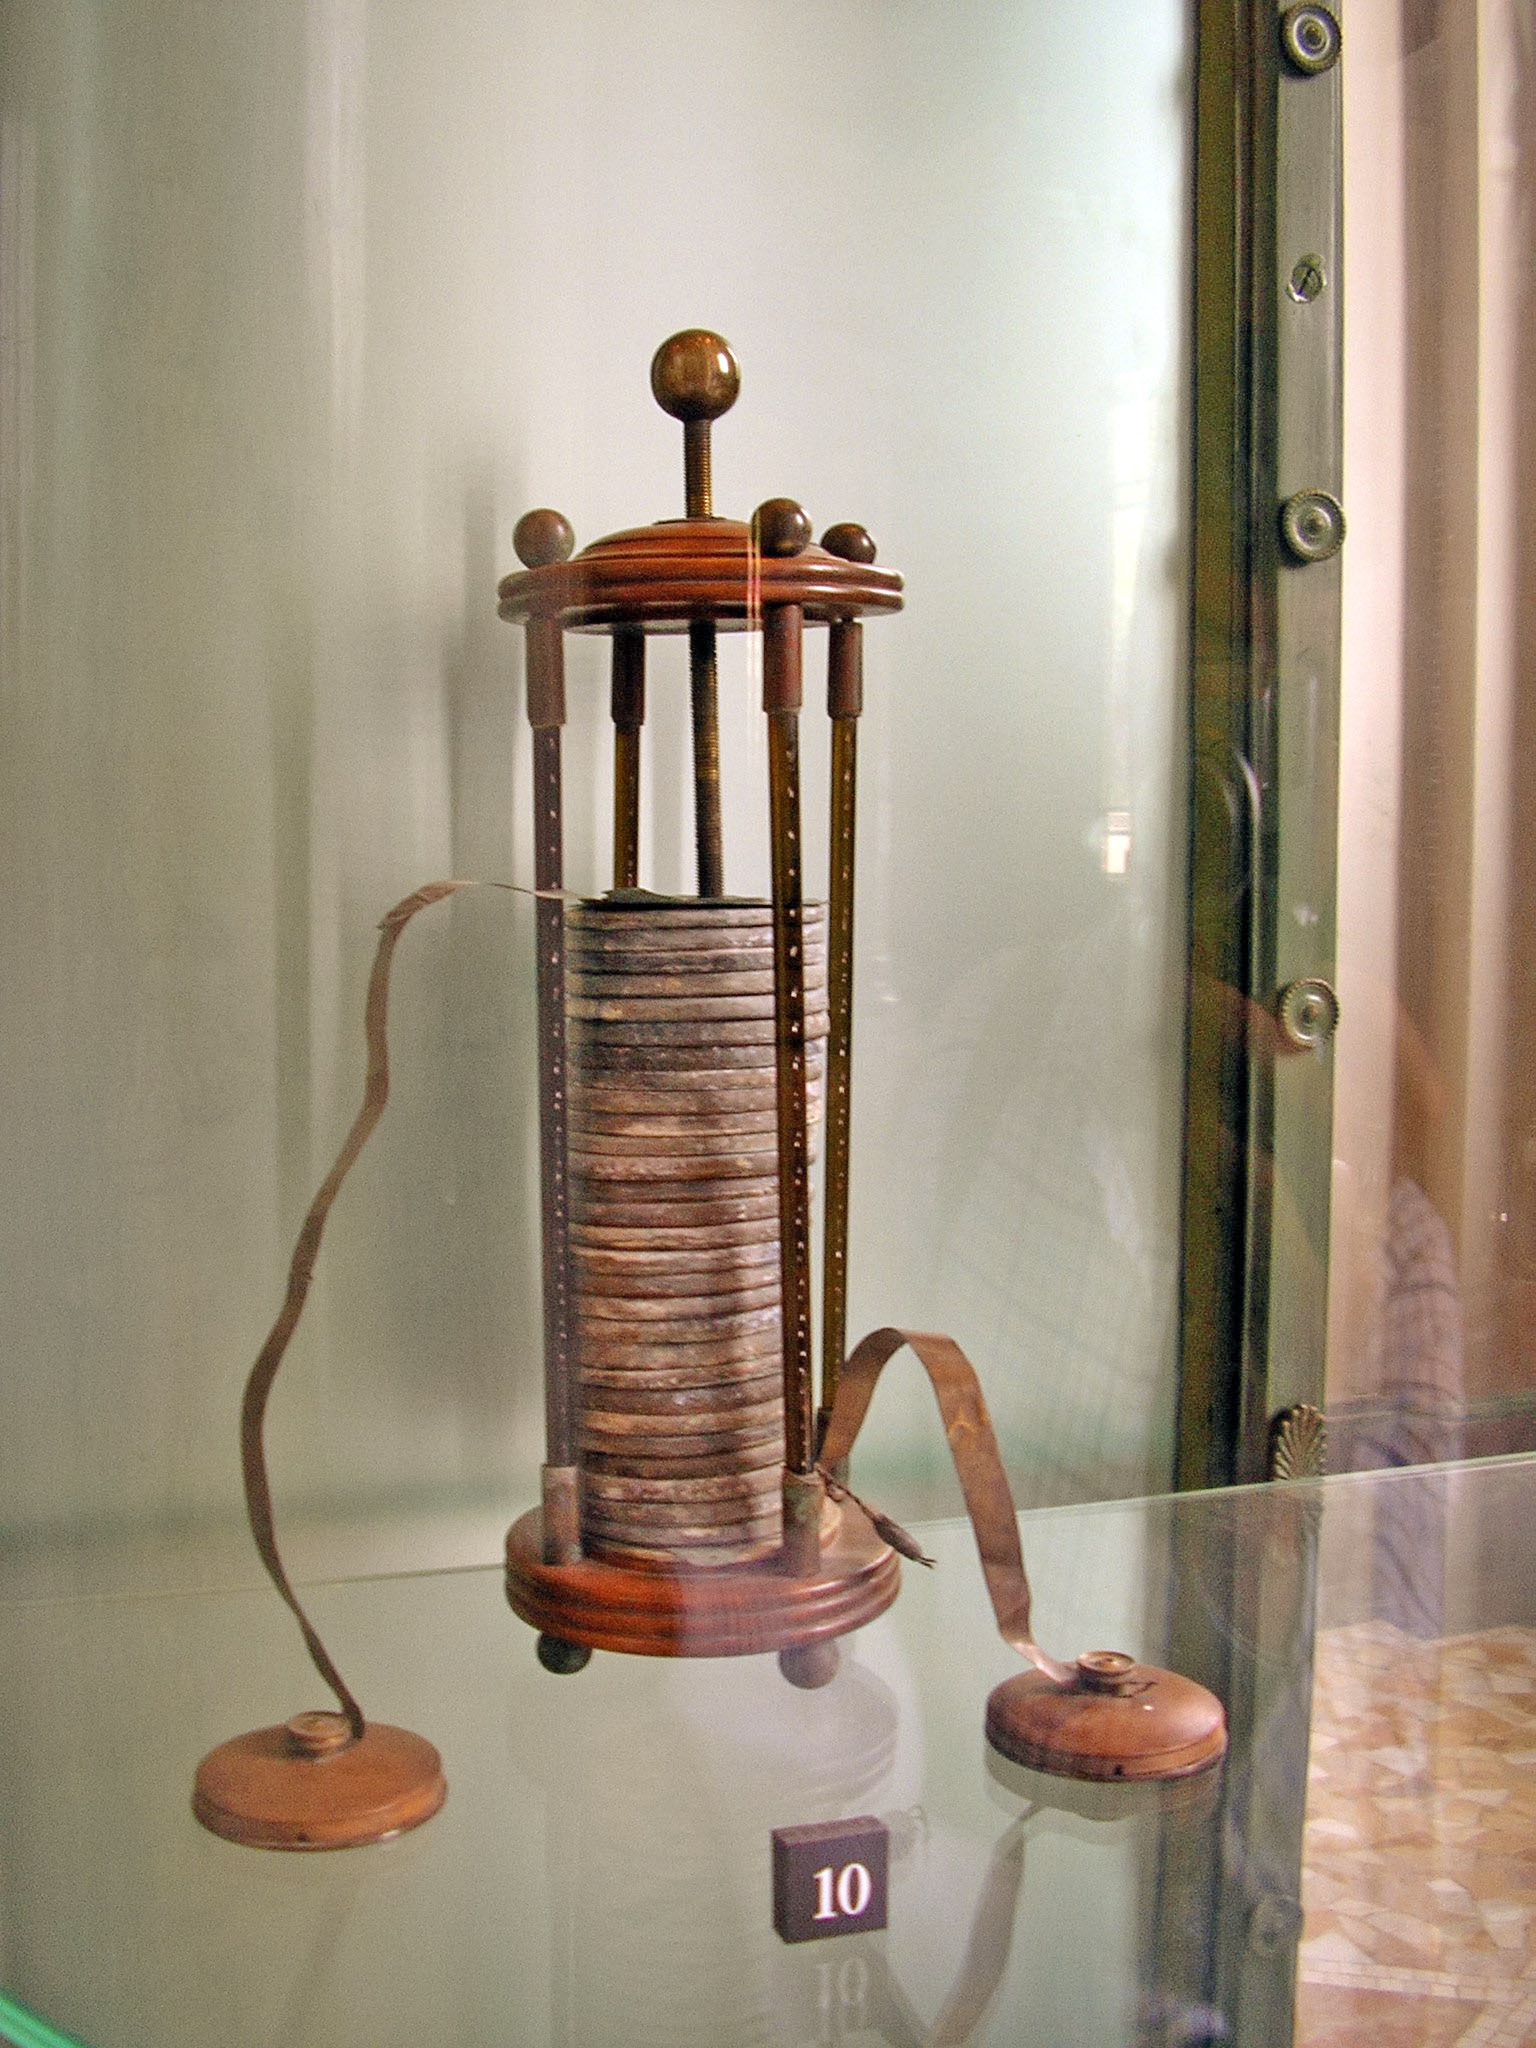
\includegraphics[width=0.24\linewidth]{images/book1/volta-pile.jpg}

{\small एक संग्रहालय में वोल्टा पुंज। फ़ोटो: गुइडोबी, CC BY-SA 3.0।}
\end{omfigure}

\section{सेल की वोल्टता}

\begin{definition}[सेल वोल्टता]\label{def:g12:cells-and-electrolysis:emf}
\emph{सेल वोल्टता}\index{सेल वोल्टता} वह वोल्टता है जो कोई धारा न देते
सेल (खुला परिपथ) के टर्मिनलों के बीच वोल्टमीटर से मापी जाती है;
यह धनात्मक होती है जब वोल्टमीटर का धनात्मक टर्मिनल
\omterm{def:g12:cells-and-electrolysis:anode}{कैथोड} पर हो।
\end{definition}

\begin{example}[डैनियल सेल]\label{ex:g12:cells-and-electrolysis:daniell}
% ledger: e0:Cu, e0:Zn, emf:Daniell
दोनों विलयन \qty{1}{mol/L} पर होने पर डैनियल सेल
\qty{1.10}{V} देता है। इलेक्ट्रोड विभवों की सारणियों से ऐसी वोल्टता का
पूर्वानुमान कैसे लगाया जाता है, यह विश्वविद्यालय के प्रथम वर्ष के खंड में दिखाया गया है।
\end{example}

\begin{remark}[सेल क्यों ख़त्म हो जाता है]\label{rem:g12:cells-and-electrolysis:runs-down}
सेल की अभिक्रिया, \ce{Zn + Cu^{2+} -> Zn^{2+} + Cu}, का स्थिरांक $K$ बहुत
बड़ा है। सेल के काम करते समय $Q = [\ce{Zn^{2+}}]/[\ce{Cu^{2+}}]$
बढ़ता है, और जब तक $Q < K$ है, अभिक्रिया चलती रहती है। जब कोई
\omterm{def:g7:chemical-reactions:reactant}{अभिकारक} समाप्त हो जाता है (जस्ता, या कॉपर \omterm{def:g9:ions:ion}{आयन}), तो धारा रुक जाती है: सेल
``ख़त्म'' हो गया है।
\end{remark}

\section{आवेश और धारिता}

\begin{definition}[फ़ैराडे स्थिरांक, धारिता]\label{def:g12:cells-and-electrolysis:capacity}
\emph{फ़ैराडे स्थिरांक}\index{फ़ैराडे स्थिरांक} $F$ \omterm{def:g9:inside-the-atom:nucleus}{इलेक्ट्रॉनों} के एक \omterm{def:g10:the-mole:amount}{मोल} का
विद्युत आवेश है, $F = N_A e = \qty{96485}{C/mol}$। किसी सेल की
\emph{धारिता}\index{धारिता} वह अधिकतम विद्युत आवेश है
जो वह दे सकता है, जिसे अक्सर ऐम्पियर-घंटों में बताया जाता है: $\qty{1}{A.h} = \qty{3600}{C}$।
\end{definition}

\begin{proposition}[आवेश और इलेक्ट्रॉनों की मात्रा]\label{prop:g12:cells-and-electrolysis:charge}
% ledger: const:F, const:NA, const:e
कोई धारा $I$, समय $\Delta t$ तक बहकर, आवेश
$Q = I\,\Delta t$ वहन करती है, अर्थात \omterm{def:g9:inside-the-atom:nucleus}{इलेक्ट्रॉनों} की यह मात्रा
\[
  n(e^-) = \frac{Q}{F} = \frac{I\,\Delta t}{F} .
\]
\end{proposition}

\begin{proof}
हर \omterm{def:g9:inside-the-atom:nucleus}{इलेक्ट्रॉन} मूल आवेश $e$ वहन करता है; \omterm{def:g9:inside-the-atom:nucleus}{इलेक्ट्रॉनों} के $n$ \omterm{def:g10:the-mole:amount}{मोल}
$n N_A e = n F$ वहन करते हैं।
\end{proof}

\begin{example}[डैनियल सेल की धारिता]\label{ex:g12:cells-and-electrolysis:capacity}
% ledger: aw:Zn, const:F
जस्ते के इलेक्ट्रोड में अभिक्रिया कर सकने वाला \qty{6.5}{g} जस्ता है, अर्थात
$6.5/65.4 = \qty{0.099}{mol}$। हर जस्ता \omterm{def:g7:atoms-and-molecules:atom}{परमाणु} दो \omterm{def:g9:inside-the-atom:nucleus}{इलेक्ट्रॉन} देता है:
$n(e^-) = \qty{0.199}{mol}$, इसलिए $Q = 0.199 \times 96485 = \qty{1.9e4}{C}$,
लगभग $\qty{1.9e4}{}/3600 = \qty{5.3}{A.h}$, यदि कॉपर \omterm{def:g9:ions:ion}{आयन} पहले
समाप्त न हो जाएँ।
\end{example}

\section{विद्युत-अपघटन}

\begin{definition}[विद्युत-अपघटन, संचायक]\label{def:g12:cells-and-electrolysis:electrolysis}
\emph{विद्युत-अपघटन}\index{विद्युत-अपघटन} किसी विद्युत जनित्र द्वारा
कराई गई वह \omterm{def:g11:redox:reaction}{अपचयोपचय अभिक्रिया} है जो उस दिशा के विपरीत चलती है जिसमें वह
अपने आप चलती। \emph{संचायक}\index{संचायक} वह सेल है जिसे
फिर से चार्ज किया जा सकता है: चार्जिंग के दौरान जनित्र उसकी अभिक्रिया को
विद्युत-अपघटन की तरह उलटी दिशा में चलाता है।
\end{definition}

\begin{inthelab}[पानी का विद्युत-अपघटन]
दो इलेक्ट्रोड थोड़े-से सोडियम सल्फ़ेट से चालक बनाए गए पानी में डूबे हैं, हर एक
विलयन से भरी एक उलटी परखनली के नीचे। कुछ वोल्ट के
जनित्र के साथ दोनों इलेक्ट्रोडों से बुलबुले उठते हैं:
\omterm{def:g12:cells-and-electrolysis:anode}{कैथोड} पर ($-$ टर्मिनल से जुड़ा) डाइहाइड्रोजन, \omterm{def:g12:cells-and-electrolysis:anode}{ऐनोड} पर
डाइऑक्सीजन, पहली गैस दूसरी से दोगुनी। \omterm{def:g4:what-a-fire-needs:burning}{जलती} तीली
पहली गैस में ``पॉप'' की आवाज़ करती है; सुलगती तीली दूसरी गैस में फिर से जल उठती है।
\end{inthelab}

\begin{omfigure}
\begin{tikzpicture}[font=\small, scale=1.2]
  % a trough of water, two inverted tubes standing in it
  \fill[omWater] (-1.4,0) rectangle (1.4,1.1);
  \foreach \x/\g in {-0.6/1.2, 0.6/0.6} {
    \fill[omWater] (\x-0.18,0.3) rectangle (\x+0.18,2.9);
    \fill[white] (\x-0.18,{2.9-\g}) rectangle (\x+0.18,2.9);
    \fill[white] (\x,2.9) circle (0.18);
    \draw[om glass] (\x-0.18,0.3) -- (\x-0.18,2.9) arc[start angle=180, end angle=0, radius=0.18] -- (\x+0.18,0.3);
  }
  \draw[om glass] (-1.5,1.25) -- (-1.4,1.15) -- (-1.4,0) -- (1.4,0) -- (1.4,1.15) -- (1.5,1.25);
  \fill[black!55] (-0.65,0) rectangle (-0.55,0.6);
  \fill[black!55] (0.55,0) rectangle (0.65,0.6);
  \node[draw, fill=white, minimum width=1.6cm, minimum height=0.45cm, font=\footnotesize] (g) at (0,-0.75) {जनित्र};
  \draw[black!70, thick] (-0.6,0) -- (-0.6,0 |- g.north);
  \draw[black!70, thick] (0.6,0) -- (0.6,0 |- g.north);
  \node[font=\footnotesize] at (-0.78,-0.3) {$-$};
  \node[font=\footnotesize] at (0.78,-0.3) {$+$};
  \node[anchor=east, align=right] at (-0.95,2.5) {डाइहाइड्रोजन\\ (कैथोड)};
  \node[anchor=west, align=left] at (0.95,2.5) {डाइऑक्सीजन\\ (ऐनोड)};
\end{tikzpicture}

{\small पानी का \omterm{def:g12:cells-and-electrolysis:electrolysis}{विद्युत-अपघटन}: इलेक्ट्रोडों के ऊपर डाइऑक्सीजन से दोगुनी
डाइहाइड्रोजन एकत्र होती है।}
\end{omfigure}


\begin{example}[पानी, विभाजित]\label{ex:g12:cells-and-electrolysis:water}
\omterm{def:g12:cells-and-electrolysis:anode}{कैथोड} पर: \ce{2H2O + 2e- -> H2 + 2OH-}; \omterm{def:g12:cells-and-electrolysis:anode}{ऐनोड} पर:
\ce{6H2O -> O2 + 4H3O+ + 4e-}। चार \omterm{def:g9:inside-the-atom:nucleus}{इलेक्ट्रॉनों} के लिए डाइहाइड्रोजन के दो \omterm{def:g7:atoms-and-molecules:molecule}{अणु}
और डाइऑक्सीजन का एक, जबकि दोनों इलेक्ट्रोडों पर बने \omterm{def:g9:ions:ion}{आयन} \ce{H3O+} और \ce{OH-}
फिर से मिलकर पानी बना लेते हैं: समग्र रूप से
\ce{2H2O -> 2H2 + O2}, जो
हाइड्रोजन के \omterm{def:g4:what-a-fire-needs:burning}{दहन} की उलटी अभिक्रिया है, और जिसे होने के लिए ऊर्जा चाहिए।
\end{example}

\begin{method}[विद्युत-अपघटन द्वारा जमा द्रव्यमान]\label{met:g12:cells-and-electrolysis:mass}
\begin{enumerate}
  \item उस इलेक्ट्रोड का \omterm{def:g11:redox:couple}{अर्ध-समीकरण} लिखिए जहाँ \omterm{def:g9:periodic-table-first-look:metal}{धातु} बनती है,
        उदाहरण के लिए \ce{Cu^{2+} + 2e- -> Cu}।
  \item आवेश $Q = I \Delta t$ और $n(e^-) = Q/F$ निकालिए।
  \item प्रति \omterm{def:g7:atoms-and-molecules:atom}{परमाणु} \omterm{def:g9:inside-the-atom:nucleus}{इलेक्ट्रॉनों} की संख्या से भाग दीजिए: $n(\ce{Cu}) =
        n(e^-)/2$; फिर $m = n \times M$।
\end{enumerate}
\end{method}


\begin{example}[ताँबे का शोधन]\label{ex:g12:cells-and-electrolysis:refining}
% ledger: aw:Cu, const:F
प्रगालक से आया अशुद्ध ताँबा कॉपर सल्फ़ेट विलयन में एक \omterm{def:g12:cells-and-electrolysis:electrolysis}{विद्युत-अपघटन} सेल का
\omterm{def:g12:cells-and-electrolysis:anode}{ऐनोड} बनाया जाता है, और शुद्ध ताँबे की एक पतली चादर \omterm{def:g12:cells-and-electrolysis:anode}{कैथोड}।
\omterm{def:g12:cells-and-electrolysis:anode}{ऐनोड} पर ताँबा \omterm{def:g2:mixing-and-dissolving:dissolve}{घुलता} है, \ce{Cu -> Cu^{2+} + 2e-}; \omterm{def:g12:cells-and-electrolysis:anode}{कैथोड} पर
शुद्ध ताँबा जमता है, \ce{Cu^{2+} + 2e- -> Cu}; अशुद्धियाँ
तली में गिर जाती हैं या विलयन में रहती हैं। \qty{24}{h} तक \qty{100}{A} की
धारा $Q = 100 \times 86400 = \qty{8.64e6}{C}$ वहन करती है, अर्थात
$n(e^-) = \qty{89.5}{mol}$, जो ताँबे के $89.5/2 = \qty{44.8}{mol}$ जमा करती है:
\qty{2.84}{kg}।
\end{example}

\begin{omfigure}
\begin{tikzpicture}[font=\small, scale=1.25]
  \pic[transform shape] at (0,0) {beaker={0.75}{cyan!70!blue!35}};
  \pic[transform shape] (an) at (-0.4,0.2) {electrode={orange!40!brown!80!black}};
  \pic[transform shape] (ca) at (0.4,0.2) {electrode={orange!80!brown}};
  \foreach \p in {(-0.6,0.08),(-0.5,0.12),(-0.3,0.07),(-0.2,0.1)} \fill[black!55] \p circle (0.03);
  \node[draw, fill=white, font=\footnotesize, minimum width=1.6cm] (g) at (0,3.4) {जनित्र};
  \draw[black!70, thick] (an-top) -- (an-top |- g.south);
  \draw[black!70, thick] (ca-top) -- (ca-top |- g.south);
  \node[font=\footnotesize] at (-0.58,2.95) {$+$};
  \node[font=\footnotesize] at (0.58,2.95) {$-$};
  \draw[omProp, thick, <-] (-0.55,1.2) -- (-1.6,1.6) node[left, align=right, text=black] {अशुद्ध ताँबे का\\ ऐनोड: घुलता है};
  \draw[omProp, thick, <-] (0.55,1.2) -- (1.6,1.6) node[right, align=left, text=black] {शुद्ध ताँबे का\\ कैथोड: बढ़ता है};
  \draw[omProp, thick, <-] (-0.35,0.1) -- (-1.6,0.3) node[left, text=black] {अशुद्धियाँ};
\end{tikzpicture}

{\small \omterm{def:g12:cells-and-electrolysis:electrolysis}{विद्युत-अपघटन} द्वारा ताँबे का शोधन: ताँबा अशुद्ध
\omterm{def:g12:cells-and-electrolysis:anode}{ऐनोड} से विलयन से होकर शुद्ध \omterm{def:g12:cells-and-electrolysis:anode}{कैथोड} तक जाता है।}
\end{omfigure}

\section{बैटरियाँ, संचायक और ईंधन सेल}

हर बैटरी एक सेल है, हर रिचार्ज होने वाली बैटरी एक \omterm{def:g12:cells-and-electrolysis:electrolysis}{संचायक}। कार का
लेड--अम्ल \omterm{def:g12:cells-and-electrolysis:electrolysis}{संचायक} सीसे, लेड ऑक्साइड और सल्फ़्यूरिक
अम्ल के साथ काम करता है; फ़ोन का लिथियम-आयन \omterm{def:g12:cells-and-electrolysis:electrolysis}{संचायक} लिथियम \omterm{def:g9:ions:ion}{आयनों} को दो
इलेक्ट्रोडों के बीच, एक ग्रेफ़ाइट का और एक किसी \omterm{def:g9:periodic-table-first-look:metal}{धातु} ऑक्साइड का, किसी द्रव
या बहुलक विद्युत-अपघट्य से होकर ले जाता है, जबकि \omterm{def:g9:inside-the-atom:nucleus}{इलेक्ट्रॉन} बाहरी
परिपथ से घूमकर जाते हैं। \omterm{def:g4:what-a-fire-needs:fuel}{ईंधन} सेल वह सेल है जिसके \omterm{def:g7:chemical-reactions:reactant}{अभिकारक} लगातार भरे जाते हैं:
हाइड्रोजन \omterm{def:g4:what-a-fire-needs:fuel}{ईंधन} सेल अभिक्रिया \ce{2H2 + O2 -> 2H2O} चलाता है, जो
पानी के \omterm{def:g12:cells-and-electrolysis:electrolysis}{विद्युत-अपघटन} की उलटी है, और विद्युत और पानी देता है।
पवन या सूर्य की विद्युत से \omterm{def:g12:cells-and-electrolysis:electrolysis}{विद्युत-अपघटन} द्वारा बनाई गई और फिर
\omterm{def:g4:what-a-fire-needs:fuel}{ईंधन} सेलों में इस्तेमाल की गई डाइहाइड्रोजन उस विद्युत को संचित करने का एक तरीका है।

\begin{omfigure}
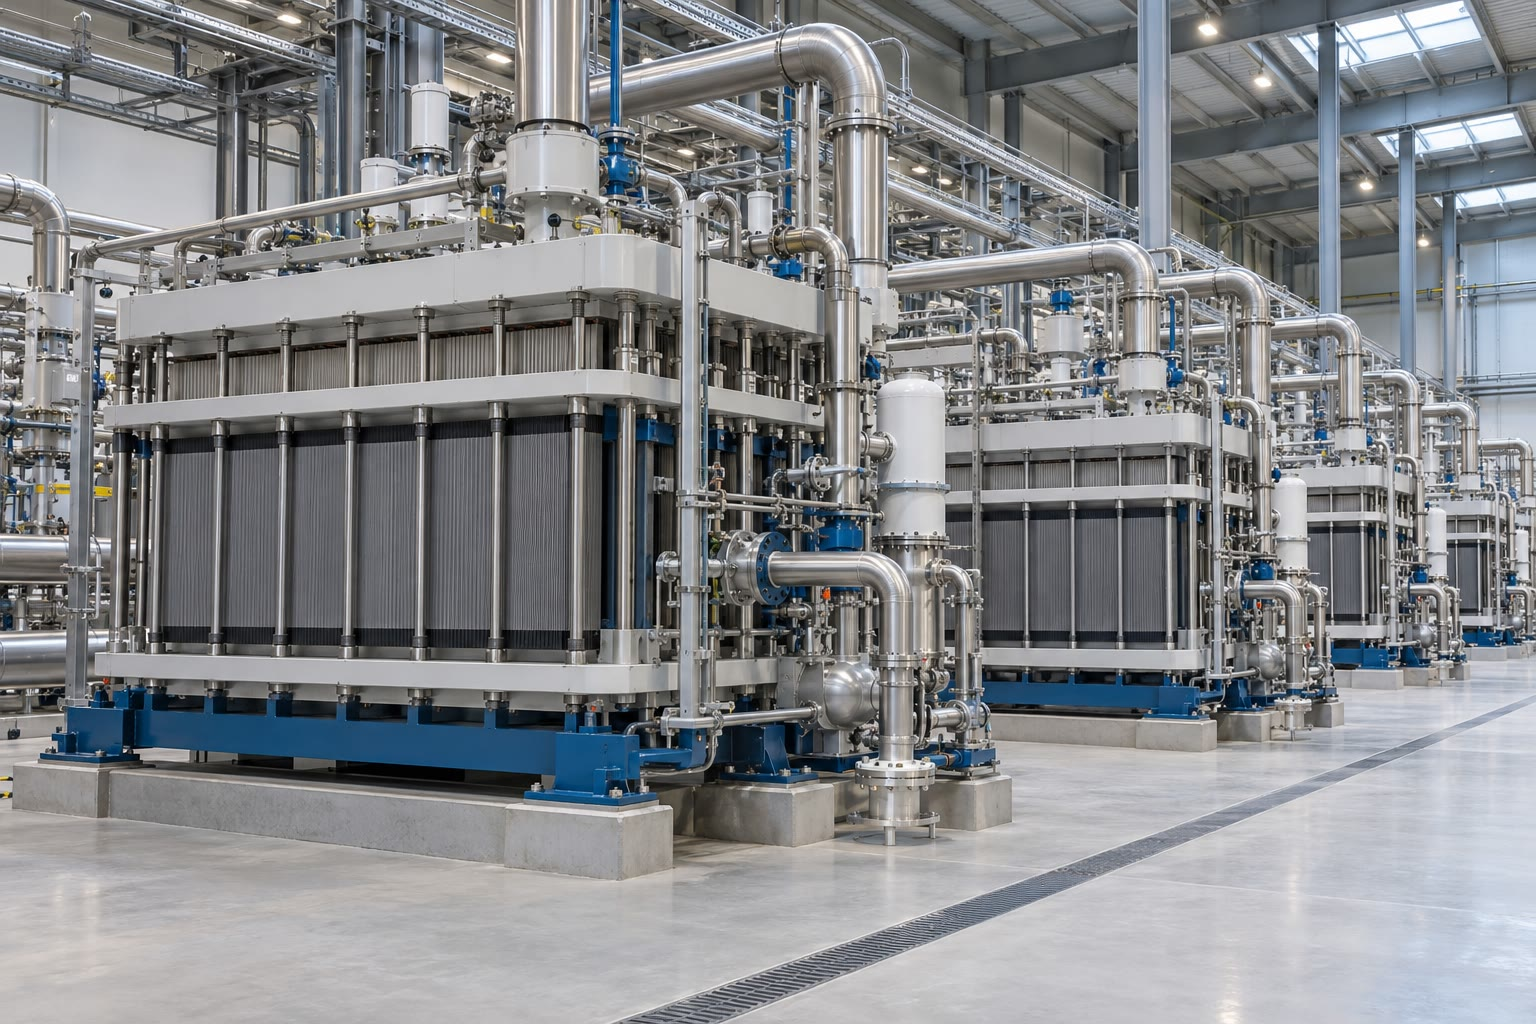
\includegraphics[width=0.48\linewidth]{images/book1/ai/g12-electrolyser-hall.jpg}

{\small एक विद्युत-अपघटक हॉल: पानी डाइहाइड्रोजन और
डाइऑक्सीजन में विभाजित होता है।}
\end{omfigure}

\section{अभ्यास}

\begin{exercise}[$\star$]\label{exo:g12:cells-and-electrolysis:1}
डैनियल सेल में कौन-सा इलेक्ट्रोड \omterm{def:g12:cells-and-electrolysis:anode}{ऐनोड} है? कौन-सा \omterm{def:g12:cells-and-electrolysis:anode}{कैथोड}? हर एक पर
\omterm{def:g11:redox:couple}{अर्ध-समीकरण} लिखिए।
\end{exercise}

\begin{exercise}[$\star$]\label{exo:g12:cells-and-electrolysis:2}
\qty{0.20}{A} की धारा \qty{30}{min} तक बहती है। वहन किया गया आवेश
और \omterm{def:g9:inside-the-atom:nucleus}{इलेक्ट्रॉनों} की मात्रा निकालिए।
\end{exercise}

\begin{exercise}[$\star$]\label{exo:g12:cells-and-electrolysis:3}
\omterm{def:g12:cells-and-electrolysis:cell}{लवण सेतु} की भूमिका क्या है? उसे हटा दिया जाए तो क्या होता है?
\end{exercise}

\begin{exercise}[$\star$]\label{exo:g12:cells-and-electrolysis:4}
\qty{2.5}{A.h} की \omterm{def:g12:cells-and-electrolysis:capacity}{धारिता} को कूलॉम में बदलिए।
\end{exercise}

\begin{exercise}[$\star$]\label{exo:g12:cells-and-electrolysis:5}
\omterm{def:g12:cells-and-electrolysis:electrolysis}{विद्युत-अपघटन} में क्या अभिक्रिया स्वतः होती है? ऊर्जा
कौन देता है?
\end{exercise}

\begin{exercise}[$\star\star$]\label{exo:g12:cells-and-electrolysis:6}
एक सेल सिल्वर नाइट्रेट में चाँदी के इलेक्ट्रोड और कॉपर सल्फ़ेट में ताँबे के
इलेक्ट्रोड से बना है। वोल्टमीटर दिखाता है कि \omterm{def:g9:inside-the-atom:nucleus}{इलेक्ट्रॉन}
ताँबे से निकलते हैं। \omterm{def:g11:redox:couple}{अर्ध-समीकरण} लिखिए, \omterm{def:g12:cells-and-electrolysis:anode}{ऐनोड} और \omterm{def:g12:cells-and-electrolysis:anode}{कैथोड} के नाम बताइए,
और समग्र अभिक्रिया दीजिए।
\end{exercise}

\begin{exercise}[$\star\star$]\label{exo:g12:cells-and-electrolysis:7}
एक घड़ी की बैटरी तीन वर्ष तक लगातार \qty{10}{\micro A} देती है।
\si{mA.h} में उसकी \omterm{def:g12:cells-and-electrolysis:capacity}{धारिता} क्या है?
\end{exercise}

\begin{exercise}[$\star\star$]\label{exo:g12:cells-and-electrolysis:8}
\qty{40}{min} तक \qty{0.50}{A} की धारा से एक चम्मच पर चाँदी की परत चढ़ाई जाती है,
\ce{Ag+ + e- -> Ag}। चाँदी का कितना द्रव्यमान जमा होता है?
\end{exercise}

\begin{exercise}[$\star\star$]\label{exo:g12:cells-and-electrolysis:9}
डैनियल सेल वाले चित्र पर तार में धारा की दिशा बताइए, और यह भी कि
सेतु के \ce{K+} और \ce{NO3-} \omterm{def:g9:ions:ion}{आयन} किस दिशा में
गति करते हैं।
\end{exercise}

\begin{exercise}[$\star\star$]\label{exo:g12:cells-and-electrolysis:10}
सेल और \omterm{def:g12:cells-and-electrolysis:electrolysis}{विद्युत-अपघटन} की तुलना कीजिए: \omterm{def:g12:cells-and-electrolysis:anode}{ऐनोड} का चिह्न, अभिक्रिया की
दिशा, ऊर्जा का रूपांतरण।
\end{exercise}

\begin{exercise}[$\star\star$]\label{exo:g12:cells-and-electrolysis:11}
पानी के \omterm{def:g12:cells-and-electrolysis:electrolysis}{विद्युत-अपघटन} में \qty{24}{mL} डाइहाइड्रोजन एकत्र की जाती है।
उसी समय डाइऑक्सीजन का कितना आयतन एकत्र होता है? क्यों?
\end{exercise}

\begin{exercise}[$\star\star\star$]\label{exo:g12:cells-and-electrolysis:12}
एक डैनियल सेल में \qty{5.0}{g} जस्ता और \qty{0.50}{mol/L} कॉपर
सल्फ़ेट के \qty{100}{mL} हैं। कौन-सा \omterm{def:g7:chemical-reactions:reactant}{अभिकारक} पहले समाप्त होता है? सेल की
\omterm{def:g12:cells-and-electrolysis:capacity}{धारिता} क्या है? यह कितने समय तक \qty{50}{mA} दे सकता है?
\end{exercise}

\begin{exercise}[$\star\star\star$]\label{exo:g12:cells-and-electrolysis:13}
\qty{1.5}{V} की एक बैटरी \qty{2.0}{A.h} देती है। उसके द्वारा संचित
ऊर्जा ($E = Q U$) जूल में और वाट-घंटों में निकालिए।
\end{exercise}

\begin{exercise}[$\star\star\star$]\label{exo:g12:cells-and-electrolysis:14}
\qty{1.0}{h} तक \qty{2.0}{A} से पानी का \omterm{def:g12:cells-and-electrolysis:electrolysis}{विद्युत-अपघटन} किया जाता है। उत्पन्न
डाइहाइड्रोजन और डाइऑक्सीजन की मात्राएँ, फिर \qty{20}{\celsius} ($V_m = \qty{24.1}{L/mol}$) पर
उनके आयतन निकालिए।
\end{exercise}

\begin{exercise}[$\star\star\star$]\label{exo:g12:cells-and-electrolysis:15}
ताँबे के शोधन में \omterm{def:g12:cells-and-electrolysis:anode}{ऐनोड} \qty{3.00}{kg} पदार्थ खोता है जबकि
\omterm{def:g12:cells-and-electrolysis:anode}{कैथोड} \qty{2.84}{kg} ताँबा प्राप्त करता है। यह मानते हुए कि \omterm{def:g12:cells-and-electrolysis:anode}{ऐनोड} पर केवल ताँबा
ऑक्सीकृत होता है और अशुद्धियाँ बस गिर जाती हैं, अशुद्ध \omterm{def:g12:cells-and-electrolysis:anode}{ऐनोड} में ताँबे का
प्रतिशत क्या है?
\end{exercise}

\section{समस्या: फ़ोन की बैटरी}

\begin{problem}[{सप्ताहांत समस्या --- \qty{4000}{mA.h} वाली फ़ोन बैटरी के इलेक्ट्रोडों के बीच
लिथियम का कितना द्रव्यमान आता-जाता है?}]
\label{pb:g12:cells-and-electrolysis:1}
% ledger: const:F, const:NA, aw:Li, dch:CH4, aw:C, aw:H
एक फ़ोन बैटरी पर अंकित है ``\qty{3.7}{V}, \qty{4000}{mA.h}''। एक
सरलीकृत चित्र में, डिस्चार्ज के दौरान ग्रेफ़ाइट इलेक्ट्रोड में संचित हर लिथियम \omterm{def:g7:atoms-and-molecules:atom}{परमाणु}
एक \omterm{def:g9:inside-the-atom:nucleus}{इलेक्ट्रॉन} देता है और लिथियम \omterm{def:g9:ions:ion}{आयन} के रूप में निकल जाता है,
\ce{Li -> Li+ + e-}; \omterm{def:g9:ions:ion}{आयन} विद्युत-अपघट्य को पार करता है और
\omterm{def:g9:periodic-table-first-look:metal}{धातु} ऑक्साइड इलेक्ट्रोड उसे ग्रहण कर लेता है, जो उसी समय एक \omterm{def:g9:inside-the-atom:nucleus}{इलेक्ट्रॉन} प्राप्त करता है।

\medskip
\noindent\textbf{भाग I --- सेल।}
\begin{enumerate}
  \item डिस्चार्ज के दौरान ग्रेफ़ाइट इलेक्ट्रोड \omterm{def:g12:cells-and-electrolysis:anode}{ऐनोड} है या
        \omterm{def:g12:cells-and-electrolysis:anode}{कैथोड}? क्यों?
  \item ऋणात्मक टर्मिनल कौन-सा है?
  \item \omterm{def:g9:inside-the-atom:nucleus}{इलेक्ट्रॉन} फ़ोन से होकर किस दिशा में जाते हैं?
        और बैटरी के भीतर लिथियम \omterm{def:g9:ions:ion}{आयन}?
  \item यह सेल एक \omterm{def:g12:cells-and-electrolysis:electrolysis}{संचायक} क्यों है?
\end{enumerate}

\medskip
\noindent\textbf{भाग II --- आवेश।}
\begin{enumerate}[resume]
  \item \qty{4000}{mA.h} को ऐम्पियर-घंटों में, फिर कूलॉम में बदलिए।
  \item यह आवेश \omterm{def:g9:inside-the-atom:nucleus}{इलेक्ट्रॉनों} की जितनी मात्रा दर्शाता है, वह निकालिए।
  \item यह कितने \omterm{def:g9:inside-the-atom:nucleus}{इलेक्ट्रॉन} हैं?
  \item फ़ोन औसतन \qty{0.25}{A} लेता है। पूरी भरी
        बैटरी कितनी देर चलती है?
  \item स्क्रीन 20 \% दिखाती है। कूलॉम में कितना आवेश बचा है?
\end{enumerate}

\medskip
\noindent\textbf{भाग III --- ऊर्जा।}
\begin{enumerate}[resume]
  \item संचित ऊर्जा, $E = Q U$, जूल में निकालिए।
  \item उसे वाट-घंटों में बदलिए।
  \item \qty{1}{g} मेथेन \omterm{def:g4:what-a-fire-needs:burning}{जलाने} पर मुक्त ऊर्जा
        (\qty{55.7}{kJ}) से तुलना कीजिए।
  \item यदि कोई ऊर्जा नष्ट न हो, तो \qty{1}{kW.h} विद्युत कितनी पूरी चार्जिंग देती
        है?
\end{enumerate}

\medskip
\noindent\textbf{भाग IV --- फिर से चार्ज करना।}
\begin{enumerate}[resume]
  \item चार्जिंग के दौरान ग्रेफ़ाइट इलेक्ट्रोड पर कौन-सी अभिक्रिया
        होती है? वह \omterm{def:g11:redox:oxidation}{ऑक्सीकरण} है या \omterm{def:g11:redox:oxidation}{अपचयन}?
  \item फिर से चार्ज करना \omterm{def:g12:cells-and-electrolysis:electrolysis}{विद्युत-अपघटन} क्यों है?
  \item चार्जर \qty{2.0}{A} देता है। पूरी तरह फिर से चार्ज करने में कम से कम
        कितना समय लगता है?
  \item एक पूरी चार्जिंग के दौरान लिथियम \omterm{def:g9:ions:ion}{आयनों} की कितनी मात्रा विद्युत-अपघट्य
        को पार करती है?
  \item उनका द्रव्यमान निकालिए।
  \item अंतिम उत्तर बताइए: एक पूरी चार्जिंग में इलेक्ट्रोडों के बीच लिथियम का कितना
        द्रव्यमान आता-जाता है?
\end{enumerate}
\end{problem}
